% !TEX root = ../Thesis.tex
\chapter{Evaluation}
\label{c:evaluation}

This chapter is separated into two sections. The first section aims to validate and verify the implementation in terms of their
correct execution. It focuses on the core contributions, such as the lazy replicaiton algorithm as well as the freshness filter capability.
Further it ensures the correct handling of the described constraints and establishes certain test cases to identify possibile failures that can occur 
during execution as well as suitable failure handling scenarios.

The second part of this chapter focuses on benchmarking the implementation on the basis of the described motivational scenario itself.
Since one of the main goals was to relax the consistency and allow 
This is followed by comparing the performance of several cases to identify how the system will behave in certain situations.
Further it will compare several executions to determine how the impleemntation affect the providede requirements.

Furthermore the performance of the individual functionalities is benchmarked and compared against slightly adjusted variations 
to give an comprehensive overview of the impact.


\section{Goal}
The evaluation has two goals the correctness as well as the impact of data freshness onto different kinds of workloads.

Verify and validate the correctness as well as the completeness of the implementation based on several characteristics.
These include the correct execution of lazy replication, the possibility to refresh statements on demand.

Impact of the replication engine on the underlying performance, if freshness indeed increases the overall parallel writes on the system.
Or if it is just marginally lower than before. Also compare this to the overall introduced overhead. And if the change was wort it



Compare underlying stores to assess the deviations of the polystore in total.
%%%%%%%%%%%%%%%%%%%%%%%%%%%%%%%%%%%%%%%%%%%%%%%%%%%%%%%%%%%%%%%%%%

\section{Correctness}

The correctness of the introduced solution mainly focuses on two parts. For one the replication behaviour, to verify if each lazy replication is carried out correctly,
and if not verify that reasonable counter measures are in place and apply them. This is crucial since we do not compare the footprint or the integrity of the data after 
a replication update. Rather we compare on a high level the metadata 
(i.e. if the number of modifications and the commit timestamp after the data replication are equal on primary and secondary node) of two replicas. 

The second part of the validation process focuses on the retrieval of outdated nodes. Although we always have a fall back to the primary placements as described in section \ref{sec:freshness_selection},
we still want to avoid excessive locking to parallelize requests to ultimately speed up the average response time.


\todo{Also checks for freshness specification if this can for one be even applied to the system , due to ongoing constraints or if it is even posssible to specify a freshness index >1.0}
\todoMissing{\ref{sec:constraints, lazy -> eager and outdated -> refreshable}}
\todoMissing{As already suggested within constrianst we have to ensure that data will not be lost}

\todoMissing{How to ensure that cached freshness objects are not falesely executed and secertly violating the specified freshness (It is rechecked)}

%%%%%%%%%%%%%%%%%%%%%%%%%%%%%%%%%%%%%%%%%%%%%%%%%%%%%%%%%%%%%%%%%%

\section{Benchmarks}



\todo{Explain why it is necessary to verify the solution with different combinations}

\subsection{Evaluation Environment}
\todo{Elaborate and thoroughly explain why the environment was chosen and how the test was executed for the sake of rerpoducibility}

If not explititly stated otherwise, the benchmarks will be executed using two underlying stores.

Define that we have HSQLDB fast and PSQL slow because on docker.

First show single Performance on the Store to see which one is the slower one of these stores in our setup.
This will also show which stores logically bound the primary transaction time. PSQL on Docker. Since Docker Containers use a limited shared set of resources 
this store immitating a slower performinh node in oru setup.


Define Workload Environement
DQL DML
Mixed Worklaod if not stated otherwise is  60\% read-operations and 40\% write-operations

\subsection{Evaluation Procedure}
The following steps outline the procedure for benchmarking data freshness within Polypheny-DB.


progressiviely build on top of each other, test after test.

\todo{Check how fast the replication is compared to the primary execution. Benchmark on two equal stores and measure the time}
\todo{ Execute benchmarks on multimodal dbs. as well as different kind of }
\todo{ Talk about implementation of freshness characteristic in many query languages}
\todoMissing{Check if freshness could even be used, or if we would always fallback to primary or when is the turining point when the freshness now works.}
\todoMissing{Schuldt FAS Evaluation possibilities}
\todoMissing{Story - konzept nicht Abstrakt und warum mit Polystore gut - mit Motivation verknüpfen}


\subsubsection{Overhead} 
Polystore systems and specifically Polypheny-DB uniformly collect all incoming requests, process them and then
route the resulting queries to the designated stores, where they will be finally executed. 
However, due to this centralized processing, addtional introduced overhead will directly impact the performance of the system.
Although, Polypheny-DB aims to provide cost- and workload-aware self-adaptiveness, to provide the best possible query results,
its internal processing is executed on top of the actual execution of the underlying store.
This can have a crucial impact on the entire throughput of the system.\\
Hence we used Chronos\todoMissing{cite} a benchmarking tool....
to measure the overhead. For this evaluation the introduced implementation is compared against the current state of Polypheny-DB.\\

As depicted in Figure \ref{fig:overhead}, the results indeed show that the implementation introduced a little overhead for single store operations.
However with multiple stores the actual average execution time was indeed slightly reduced. Although, single store executions should not be entirely negelcted
they do not form the main pursuit of polystore systems, which are more suitably visualized by the multistore runtime.

\todoMissing{Contain overhead as much as possible otherwise the freshness eveluation will negativiely impact regular operations}

\begin{figure}[t] 
    \centering 
    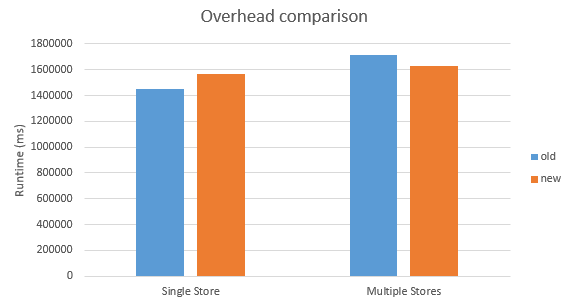
\includegraphics[width=0.7\textwidth]{Figures/overhead.png}
    \caption{Overhead comparison of the entire implemation.}
    \label{fig:overhead}
\end{figure}

%%%%%%%%%%%%%%%%%%%%%%%%%%%%%%%%%%%%%%%%%%%%%%%%%%%%%%%%%%%%%%%%%%

\subsubsection{Locking } 

As described in Section \ref{sec:strategy}, one of the prerequisites to establish multiple refresh strategies and hence lazy replication,  
was the refactoring of the locking mechanism. Although, not completely reworked, the locking-module of Polyphenys SS2PL 
poses as a core component of the system. It therefore  impacts correct serializability treatement and is and inherent driver of 
the concurrency which directly influences the overall performance of the system.\\
For the evaluation again the current state of Polypheny-DB is compared against this implementation.
Since the locking module was changed from a table-wise locking towards a partition-wise locking we will validate the impact on the basis of 
a single table using YCSB\todoMissing{cite}. 
The evaluation was executed with gradually increasing numbers of partitions, which are placed on one store or distributed across $n$-Stores 
for $n$ partitions to observe any changes on the locking and therefore the throughput.\\
To get a general overview of the impact, the benchmark was executed using a mixed workload.\\

\begin{figure}
    \centering
    \begin{subfigure}{.5\textwidth}
      \centering
      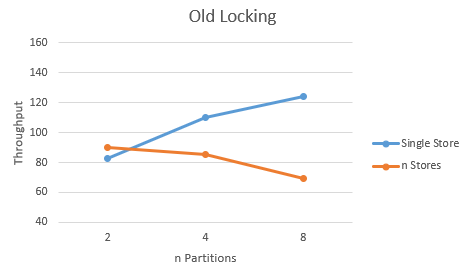
\includegraphics[width=.7\linewidth]{Figures/old_locking.PNG}
      \caption{Old Locking}
      \label{fig:oldlock}
    \end{subfigure}%
    \begin{subfigure}{.5\textwidth}
      \centering
      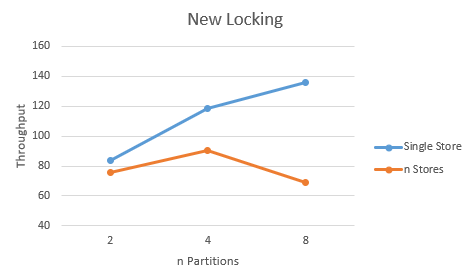
\includegraphics[width=.7\linewidth]{Figures/new_locking.PNG}
      \caption{New Locking}
      \label{fig:newlock}
    \end{subfigure}
    \begin{subfigure}{.7\textwidth}
        \centering
        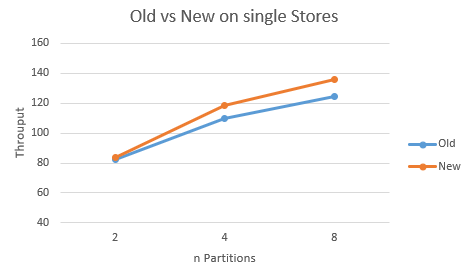
\includegraphics[width=.7\linewidth]{Figures/old_vs_new.PNG}
        \caption{Old vs. New Locking}
        \label{fig:oldandnewlock}
      \end{subfigure}
    \caption{A figure with three subfigures}
    \label{fig:lock_comp}
\end{figure}

As visualized in Figure \ref{fig:oldlock} and \ref{fig:newlock}, for both cases the overall situation is quite similiar.
While the distribution of the partitions across several stores gets gradually worse, the single store performance actually improves the more partitions are added to the table.
This behaviour is essentially caused by the Polyphenys need to join and union several stores together, when querying multiple partitions across several stores.
Since more stores need to be connected and considered, it is a rather costly approach and as stated before gets increasingly harder the more stores are involved.\\

Because the single store variations prove to be more reliable, they are summarized in \ref{fig:oldandnewlock}.
We can observe that the new locking mechanism indeed proves to be slightly better in terms of the possible throughput.
Furthermore it shows that again with a growing number of stores, the gap between the old and new locking extends even more, validating the benefits of the new locking mechanisms.




%%%%%%%%%%%%%%%%%%%%%%%%%%%%%%%%%%%%%%%%%%%%%%%%%%%%%%%%%%%%%%%%%%


\subsubsection{Baseline Identification} 
\todoMissing{Single PSQL vs HSQL}

Since the Lazy Replication algorithm is not only fundamental to generate multiple versions to be used within freshness-awareness
but also a core functionality how data is propagated throughout the system. 
Hence, along with the newly introduced replication strategies, and \emph{Change Data Collection} it will have a major impact on the overall perfromance of the system.
Since the replication solely focuses on replicating captured changes, the next benchmarks will be consequently executed using only DML-operations without any reads.\\

\begin{figure}[t] 
    \centering 
    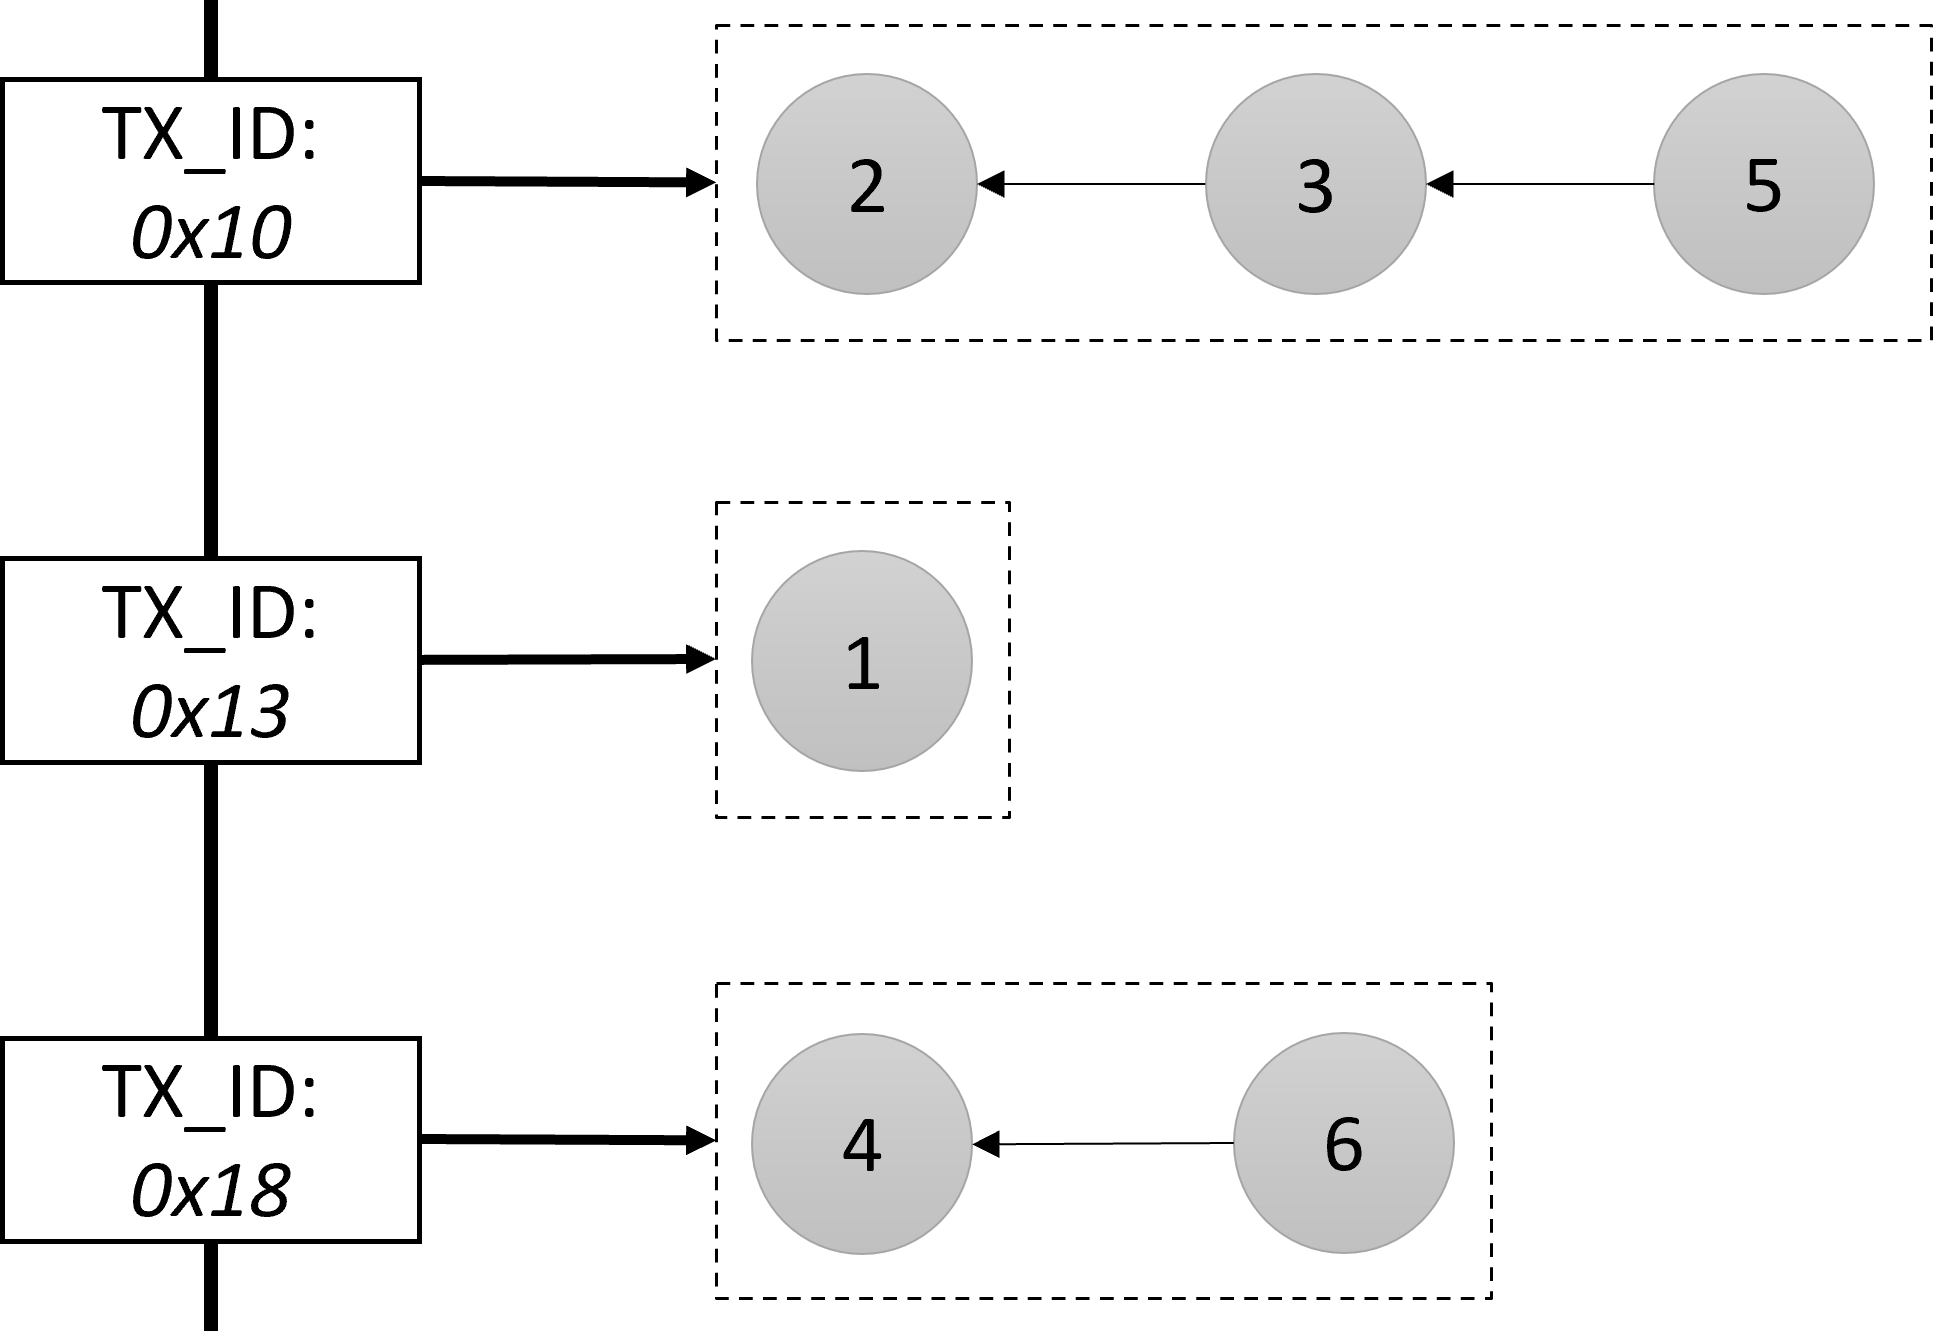
\includegraphics[width=0.7\textwidth]{Figures/store_comparision.png}
    \caption{Single DML PostgreSQL vs. Single HSQLDB}
    \label{fig:singlepsqlhsql}
\end{figure}

As stated in the evaluation environement \todoMissing{ref section}, these benchmarks will be mainly executed with HSQLDB and PostgreSQL running within a virtualized 
container environment. To have a general base line for comparison Figure \ref{fig:singlepsqlhsql} presents a single store execution, comparing theses two stores against each other.
As motivated in the beginning, it is crucil for a system to utilize the key benefits of each store. For our scenario this is important to determine which 
store configuration is more suitable to be used as an eagerly replicated priamry placement, due to its lower latency and better reponse time.\\
This illustreated comparison clearly shows that Due to its limited resources the PostgreSQL store cannot directly compete with this HSQLDB configuration.
This provides us with the intuitive decission to use HSQLDB for the priamry transactions.




%%%%%%%%%%%%%%%%%%%%%%%%%%%%%%%%%%%%%%%%%%%%%%%%%%%%%%%%%%%%%%%%%%




\subsubsection{Lazy Replication} 
\todoMissing{TERMINAL 1 vs TERMINAL 50 }

As previously stated, the replication strategies will impact the processing capability of the system immensly.
A placement with a configured lazy replication strategy automatically enables the system, to start tracking changes for this entity, impacting the duration of a query.
Therfore we want to compare how each store handles the replication differently. Consequently we want to benchmark and compare two equal placements that are eagerly replicated
against the same two stores but one configured as \emph{lazy}.\\

To extend the baseline discovered before, we again want to demonstrate the behaviour a purely sequential environment with only one client has, 
against a parallel environment with 50 clients.\\
Figure \ref{fig:terminal} shows the evaluation across two stores, providing the possible throughput per second. Which is given as the number of modifications that can be 
applied to the system per second. As before HSQLDB obviously achieves better results then PostgreSQL. However what is surprising is that disregarding the store,
and not, apparent when only considering  \ref{fig:terminal50}, the eagerly replicated configuration performs much better in all tests.
Considering that he collection of changes within a llazy setup, indeed imposes additional costs on the processing time, such deviations are expected.

\begin{figure}
    \centering
    \begin{subfigure}{.5\textwidth}
      \centering
      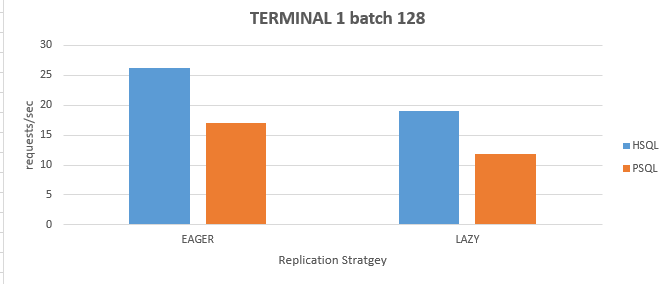
\includegraphics[width=.9\linewidth]{Figures/terminal1.PNG}
      \caption{One process}
      \label{fig:terminal1}
    \end{subfigure}%
    \begin{subfigure}{.5\textwidth}
      \centering
      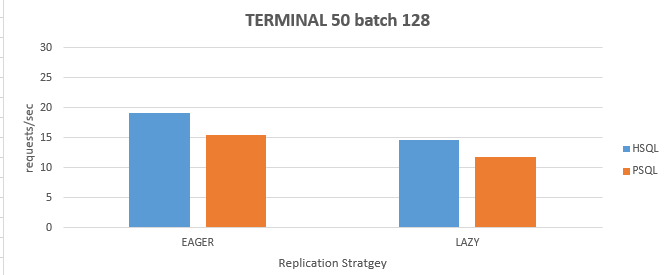
\includegraphics[width=.9\linewidth]{Figures/terminal50.PNG}
      \caption{50 processes}
      \label{fig:terminal50}
    \end{subfigure}
    \caption{Concurrency Comparison}
    \label{fig:terminal}
\end{figure}


Admittingly an enitity that is composed of only similiar or equal stores, will not be beneficial for a polystore system, to allow different workloads.
Therefore the follwoing benchmarks will concentrate on a mixed setup with interleaved stores. Furthermore these tests will be executed with 50 parallel clients to repoduce a 
conventional environment. 

%%%%%%%%%%%%%%%%%%%%%%%%%%%%%%%%%%%%%%%%%%%%%%%%%%%%%%%%%%%%%%%%%%

\todoMissing{PSQL vs HSQL DML only} 

Now focussing on a mixed setup of two stores containing PostgreSQL as well as HSQLDB for one entity.
Nativiely fo a polystore environment we want to identify which setup will produce better results, hence is suitable for which situation.
Consequently we want to observe how the order of the stores imapcts the response time per benchmark.\\
Again to have a foundation to compare our changes to we will compare the configurations if both stores are defined as eager and Further
respectiviely define each store as lazy as well.\\
Ultimately \ref{fig:psqlhsqlresponse} shows that regarding the lazy approaches, we again see the common behaviour that HSQLDB performs a little better as an eagerly replicated
store compared to PostgreSQL.
Additionally the Figure in \ref{fig:overall_comp} puts the average latency in perspective to the execution times described before.
AS one can observe the eager replications again pefrom the best while the PostgreSQL variation posing a eager perfroms the worst.
This not only allows to compare the different setups but again aids us to choose suitable combinations for our designated tasks.\\

\begin{figure}[t] 
    \centering 
    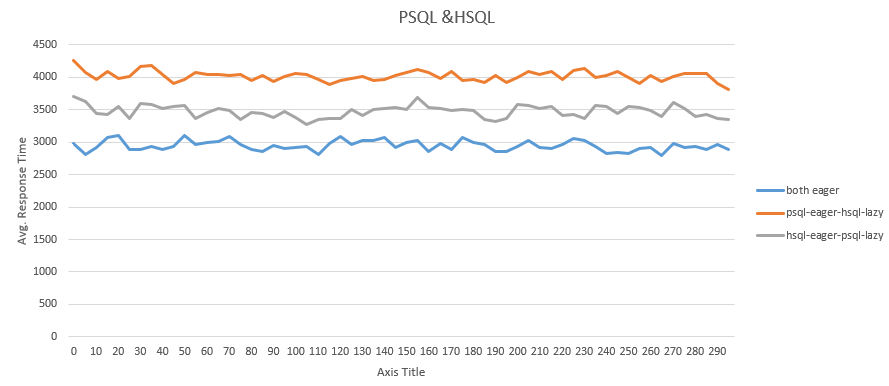
\includegraphics[width=0.7\textwidth]{Figures/PSQ_HSQL_DML_only.PNG}
    \caption{DML only - Avg. Latency comparsion PostgreSQL vs. HSQLDB. With switching Roles}
    \label{fig:psqlhsqlresponse}
\end{figure}

\begin{figure}[t] 
    \centering 
    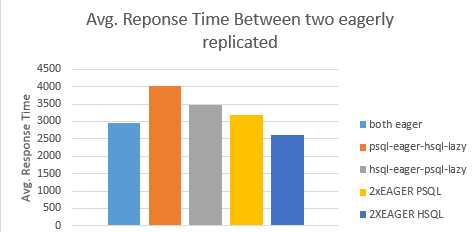
\includegraphics[width=0.7\textwidth]{Figures/psq_hsql_avg.response2.PNG}
    \caption{DML onlyAvg. Response Time Comparison of 2 store sizes and swithcing Roles}
    \label{fig:overall_comp}
\end{figure}


However, the presented possibilities so far only considered the execution on two stores. Therefore, \ref{fig:24storecomp} aims
to compare the execution on two and four stores. Again this is done in an interleaved fashion, switching the role of lazy and eager strategy between the participating stores.
During theses tests only one is eagerly replicated the remaining are all configured as lazy placements. Eagerly and lazily replicated stores in this scenario are inherently
defined to be different stores.\\
The graphs indicate that although they differ in terms of average response times, the gap between both configurations is comparably equal.
In both cases the execution with the eagerly replicated HSQLDB is roughly 500ms faster in terms of the average response time.\\


\begin{figure}
    \centering
    \begin{subfigure}{.5\textwidth}
      \centering
      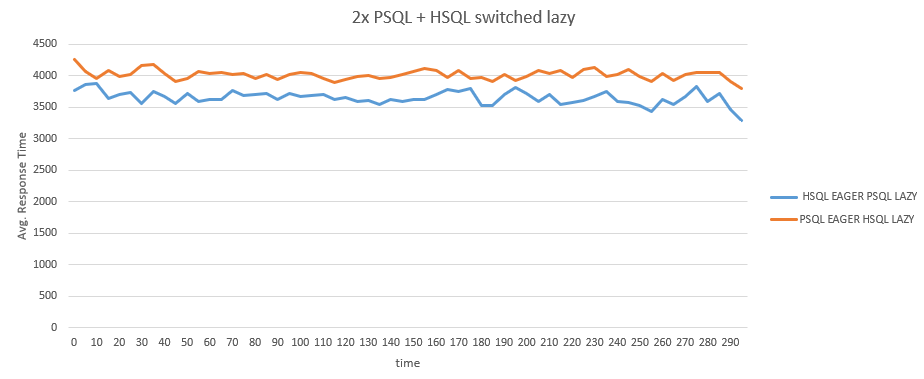
\includegraphics[width=.9\linewidth]{psql_hsql_switched_lazy.PNG}
      \caption{Comparison of 2 Stores HSQLDB and PostgreSQL. Switching Roles.}
      \label{fig:2store}
    \end{subfigure}%
    \begin{subfigure}{.5\textwidth}
      \centering
      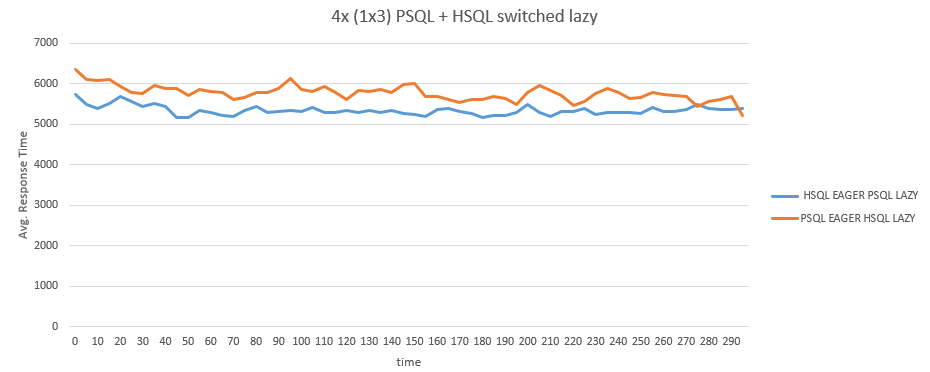
\includegraphics[width=.9\linewidth]{Figures/4psql_hsql_switched_lazy.PNG}
      \caption{Comparison of 4 Stores HSQLDB and PostgreSQL. Switching Roles.}
      \label{fig:4store}
    \end{subfigure}
    \caption{Comparison of different store sizes and swithcing Roles}
    \label{fig:24storecomp}
\end{figure}


\begin{figure}[t] 
    \centering 
    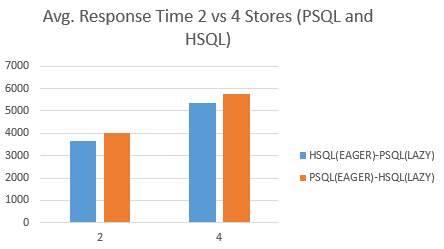
\includegraphics[width=0.7\textwidth]{Figures/24_avg_psql_hsql_switched_lazy.PNG}
    \caption{Avg. Response Time Comparison of different store sizes and swithcing Roles}
    \label{fig:24storecomp_avg}
\end{figure}


As summarized and visualized more densely in Figure \ref{fig:24storecomp_avg},
its rather counter intuitive that the configurations in \ref{fig:24storecomp} (a) and (b) deviate at all. 
In general they both only contain one primary placement that is even targeted for the primary transaction. 
However, as described before, the primary transaction is responsible for capturing, as well as queing the changes to be replicated asynchronously.
While the procedure is always executed equally, the second approach with four stores, has more replication targets that require the change. 
Since the generation of replication objects as well as the queueing are all still done during the commit of the priamry transaction, the observed
deviations are reasonable.\\




Based on this observation we specifically wanted to compare how a growth in stores will impact this deviation.
To have a more uniform result this test will be executed with two HSQLDB stores, to have a simple foundation to compare each deviation .
Without a secind store chararcteristic that could interfere with the final result.\\
In this evaluation \ref{fig:stores_comp} illustrates, the average response time of two to eight stores, where one store is eagerly replicated and the rest
is configured as lazy.






HSQL only
Compare execution time with different number of stores 1 Eager n Lazy   
(Because for Lazy there 
are more replications to put into the queue per pending operation)
Check the average repsonse Time
\begin{figure}[t] 
    \centering 
    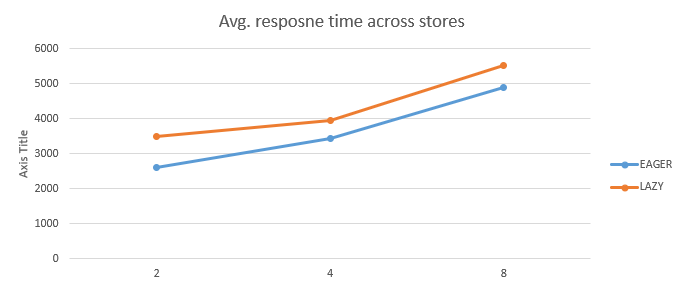
\includegraphics[width=0.7\textwidth]{Figures/hsql_avg_response_stores.PNG}
    \caption{DML only multiple STore comparison  Response Time}
    \label{fig:stores_comp}
\end{figure}


\subsubsection{Queue Replication}
Mixed 60-40

Shows the impact the queu operations have on the overall performance


As ellaborated and suggested multiple times before, the deviation between eagerly and lazily replicated deviates quite a bit.
Therefore we want to identify per operation what actuallay influences the lower resposne time.

\begin{figure}[t] 
    \centering 
    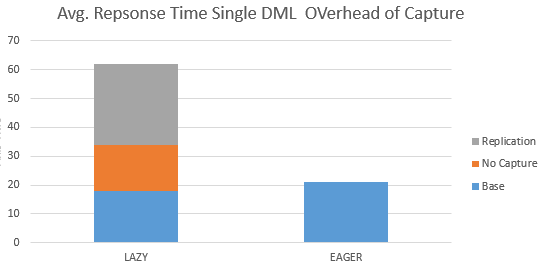
\includegraphics[width=0.7\textwidth]{Figures/dml_comp.PNG}
    \caption{Execution-Time comparision of a decompossed  single write-operation with and without data active data capture }
    \label{fig:write_decomposition}
\end{figure}


Therefore show how this deviates in General. What happens if we disable the replication queue or teh capture in geenral.
To immitate an on-demand processing where entities and placements are purposely kept at a given point

We see exactly the delay starting after 1 5se minute because afterwards the first placement could fulfil the freshness request and had to fallback to the primary who have might been locked
This graph exactly corresponds to the graph depicted in \ref{fig:write_decomposition} 
Mixed 60-40
\begin{figure}[t] 
    \centering 
    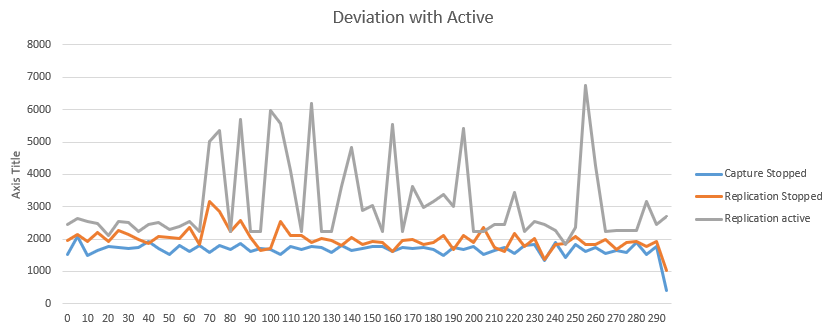
\includegraphics[width=0.7\textwidth]{Figures/deviation_with_active_que.PNG}
    \caption{Mixed Workload 60-40 with 100\% Freshness with relative read 1 minute }
    \label{fig:replication Impact}
\end{figure}








%%%%%%%%%%%%%%%%%%%%%%%%%%%%%%%%%%%%%%%%%%%%%%%%%%%%%%%%%%%%%%%%%%


\subsubsection{Compare Total Replica Convergence Time DML only } 

BOTH eager  -- PSQL EAGER HSQL LAZY -- HSQL EAGER PSQL --LAZY
In terms of their execution and replication time which one finishes faster
Also does the numbe rof stores have an impact
Mixed Worklaod?

\begin{figure}[t] 
    \centering 
    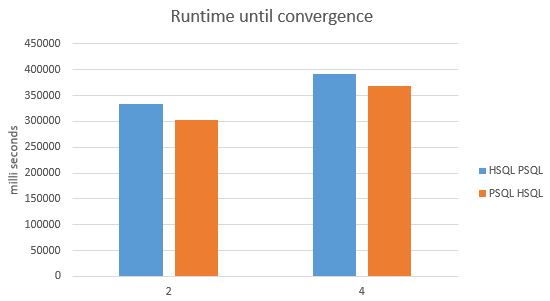
\includegraphics[width=0.7\textwidth]{Figures/runtime_convergence24.PNG}
    \caption{Convergence Time of PostgreSQL and HSQLDB with n-number of stores.}
    \label{fig:store_comparision}
\end{figure}


Average Repsonse Time accumulated with the Extension of teh Replicaiton Queue as well as the shrinking
to mimic the convergence time. 


\begin{figure}
    \centering
    \begin{subfigure}{.5\textwidth}
      \centering
      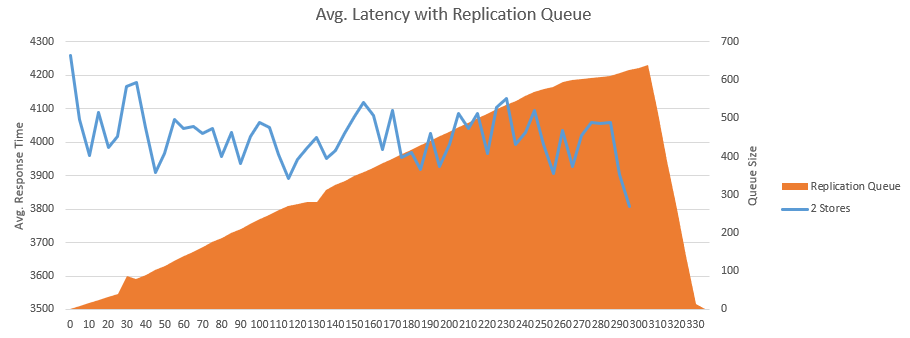
\includegraphics[width=.9\linewidth]{Figures/2latency_queue.PNG}
      \caption{2 Stores}
      \label{fig:converge_2}
    \end{subfigure}%
    \begin{subfigure}{.5\textwidth}
      \centering
      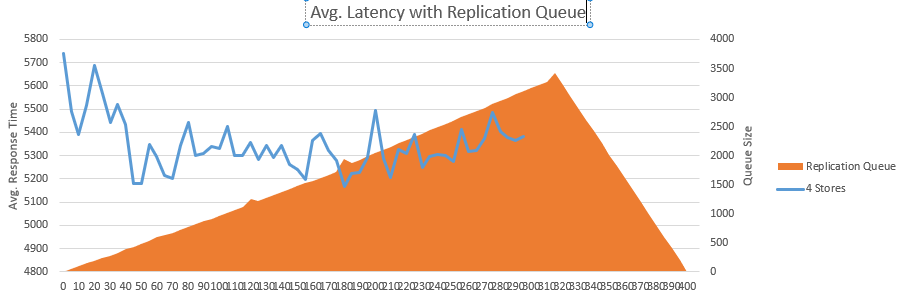
\includegraphics[width=.9\linewidth]{Figures/4latence_queue.PNG}
      \caption{4 Stores}
      \label{fig:converge_4}
    \end{subfigure}
    \caption{Execution Time and Replication Convergence}
    \label{fig:converge_24}
\end{figure}




\begin{figure}[t] 
    \centering 
    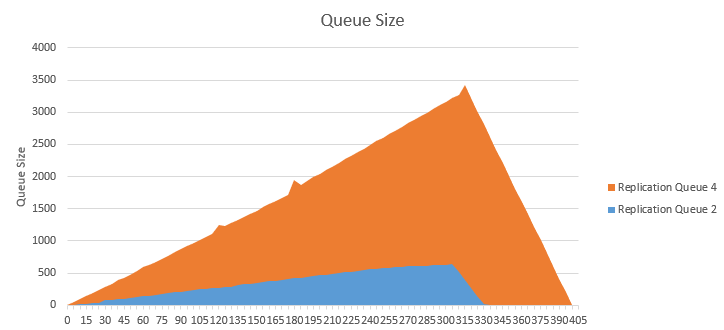
\includegraphics[width=0.7\textwidth]{Figures/queuesize24.PNG}
    \caption{Replication Queue Convergence}
    \label{fig:converge24}
\end{figure}





%%%%%%%%%%%%%%%%%%%%%%%%%%%%%%%%%%%%%%%%%%%%%%%%%%%%%%%%%%%%%%%%%%




\subsection*{Reponse Time DQL in General}

DQL only

Even with mixed workload without freshness as illustrated in Figure \ref{fig:dqldml_no_fresh}, it is obvious 
we see that the store consteallation does have an impact on the overall latency.
Whereas no freshness queries will always target the primary playement we see
again that the store with HSQLDB as a priamry node is slightly faster than the PostgreSQL Eager variation. This again proves the
point that the Store selection will have an impact.
However know compared to a query with freshness, we essentially see very flipped roles.
. This is essentially caused by the target of the select statetemntes. Since we are ratehr in a 
read-heavy environemnt the select to have quite the impact on the final result.
in contrast \ref{fig:fresh10}in that case targeting the secondary node. Where again the lazy replicated HSQL Node is better

\todoMissing{Compare with both EAGER}
No Freshness 
\begin{figure}[t] 
    \centering 
    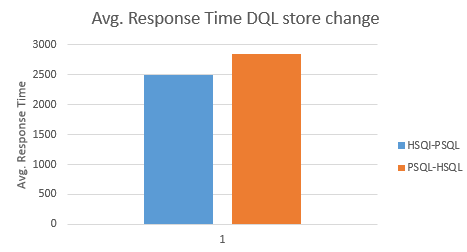
\includegraphics[width=0.7\textwidth]{Figures/avg_response-hsql-psql-dql_no_fresg.PNG}
    \caption{Mixed Workload 60-40 No freshness}
    \label{fig:dqldml_no_fresh}
\end{figure}


100 \% Freshness
\begin{figure}[t] 
    \centering 
    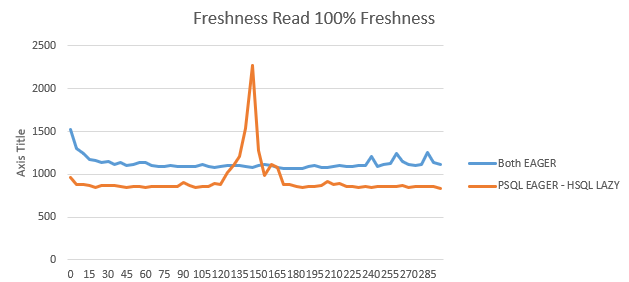
\includegraphics[width=0.7\textwidth]{Figures/100_fresh_dql.PNG}
    \caption{DQL 100\% Freshness }
    \label{fig:fresh100}
\end{figure}


\todoMissing{Introduce 0\% Freshness}
DQL 50\% Freshness
\begin{figure}[t] 
    \centering 
    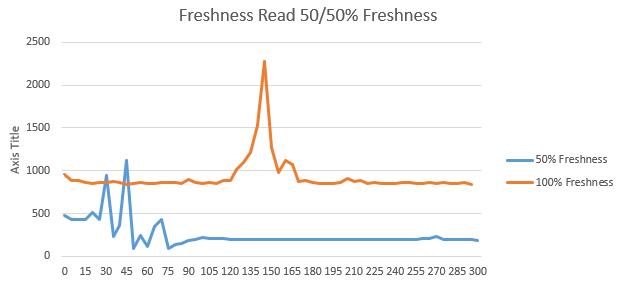
\includegraphics[width=0.7\textwidth]{Figures/50_fresh_dql.PNG}
    \caption{DQL 50\% Freshness}
    \label{fig:fresh50}
\end{figure}





%%%%%%%%%%%%%%%%%%%%%%%%%%%%%%%%%%%%%%%%%%%%%%%%%%%%%%%%%%%%%%%%%%
\subsubsection{Freshness Evaluation Type Filter} 
Show how each filter impacts the store differently, but all in all roughly the same
\begin{figure}[t] 
    \centering 
    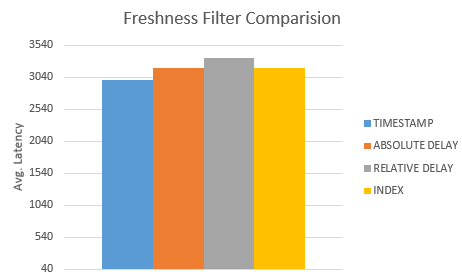
\includegraphics[width=0.7\textwidth]{Figures/freshness_comp.PNG}
    \caption{Avg. Response Time comparison of the available Evaluation Type Filter Functionality }
    \label{fig:eval_type}
\end{figure}


%%%%%%%%%%%%%%%%%%%%%%%%%%%%%%%%%%%%%%%%%%%%%%%%%%%%%%%%%%%%%%%%%%
\subsubsection{Mixed Worklaod} 

\begin{figure}[t] 
    \centering 
    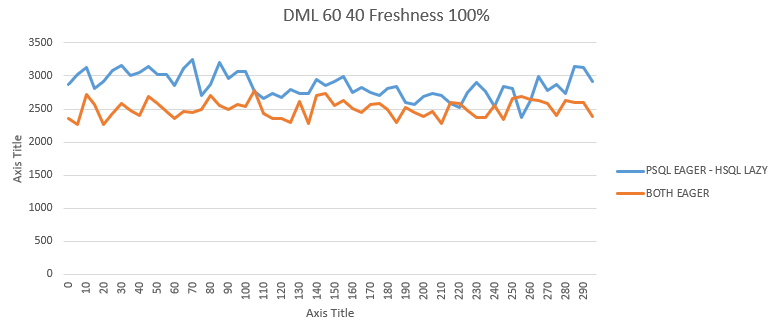
\includegraphics[width=0.7\textwidth]{Figures/60_40_fresh_100.PNG}
    \caption{60 R 40 W 100\% Freshness}
    \label{fig:}
\end{figure}




Show that the workload has a direct impact on the performance
\begin{figure}[t] 
    \centering 
    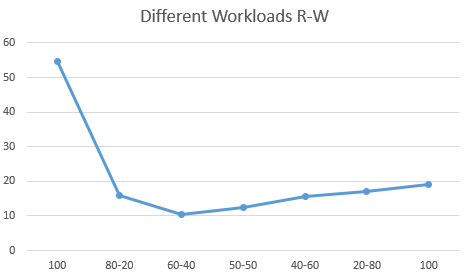
\includegraphics[width=0.7\textwidth]{Figures/different_ workloads.PNG}
    \caption{}
    \label{fig:}
\end{figure}

%%%%%%%%%%%%%%%%%%%%%%%%%%%%%%%%%%%%%%%%%%%%%%%%%%%%%%%%%%%%%%%%%%
%%%%%%%%%%%%%%%%%%%%%%%%%%%%%%%%%%%%%%%%%%%%%%%%%%%%%%%%%%%%%%%%%%
%%%%%%%%%%%%%%%%%%%%%%%%%%%%%%%%%%%%%%%%%%%%%%%%%%%%%%%%%%%%%%%%%%





\subsection{Results}
\label{sec:discussion}

The result generally shows
%%%%%%%%%%%%%%%%%%%%%%%%%%%%%%%%%%%%%%%%%%%%%%%%%%%%%%%%%%%%%%%%%%




